\documentclass[]{report}
\usepackage{graphicx} % Required for inserting images
\usepackage[T1]{fontenc}
\usepackage{courier}
\usepackage{xcolor}
\usepackage[fontsize=12pt]{scrextend}
\usepackage[a4paper, total={6in, 8in}]{geometry}
\usepackage[
    usetikz=false,
    highlight=false,
    highlightcolor=green!50!white,
    linecolor=green!20!black
]{soup}
%\usepackage{ragged2e}
\usepackage[hidelinks]{hyperref}
\usepackage{caption}
\usepackage{subcaption}
\usepackage[basque]{babel}
\usepackage{pdfpages}

\usepackage{everysel}
\renewcommand*\familydefault{\ttdefault}
\EverySelectfont{%
\fontdimen2\font=0.4em% interword space
\fontdimen3\font=0.2em% interword stretch
\fontdimen4\font=0.1em% interword shrink
\fontdimen7\font=0.1em% extra space
\hyphenchar\font=`\-% to allow hyphenation
}
\usepackage{tgcursor}

\title{KaixoMundua[0]}
\author{Software Libre Taldearen fanzinea}
\date{Fedibertsoan, 2025eko Azaroan}

\makeatletter
\newcommand\footnoteref[1]{\protected@xdef\@thefnmark{\ref{#1}}\@footnotemark}
\makeatother


\begin{document}

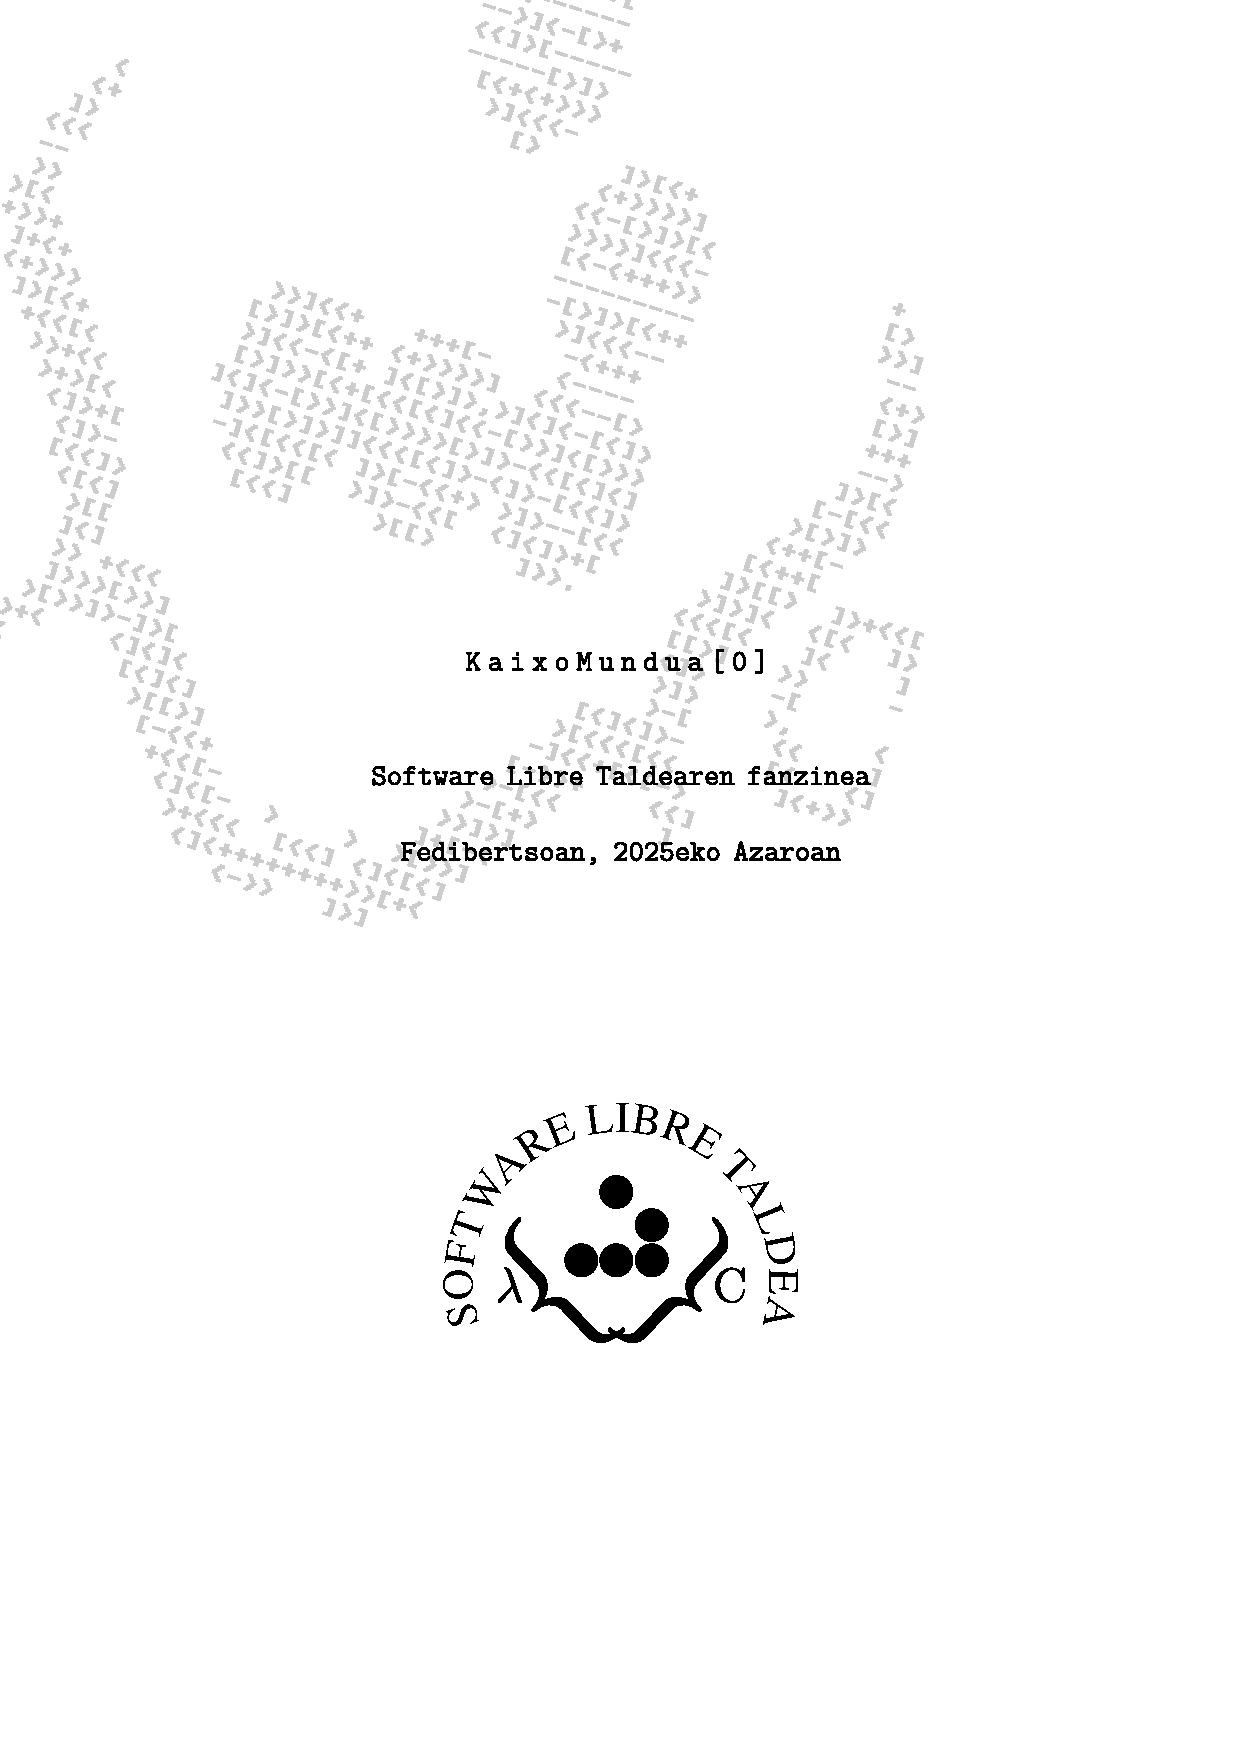
\includepdf[pages={1}]{PORTADA.pdf}

\selectfont

\pagenumbering{gobble}
\fontfamily{lmtt}\selectfont
\renewcommand{\rmdefault}{lmtt}

% \maketitle

\section*{Chat control: segurtasunaren izenean, pribatutasunaren amaiera}

%Buf a pasao una movida todo guapa (no tan guapa)

%https://www.euronews.com/next/2025/10/11/chat-control-on-hold-europes-eastern-flank-remains-passive - Artikulo

%https://www.argia.eus/albistea/whatsapp-mezuak-enkriptatzeak-ez-luke-zentzurik-europak-lege-hau-onartzen-badu - Artikulo

%https://maldita.es/malditobulo/20251015/chat-control-acceso-mensajes-ue-2025/ - Artikulo

%https://www.Internetsociety.org/wp-content/uploads/2020/03/2022-Client-Side-Scanning-Factsheet-EN.pdf - Client side scanning arriskuak

%https://edri.org/our-work/most-criticised-eu-law-of-all-time/ - Jendia haserre.

%https://csa-scientist-open-letter.org/Sep2025 - Zientzilariak haserre.

%https://x.com/wcathcart/status/1975399141527474180 - Facebook haserre XD

%https://www.patrick-breyer.de/en/posts/chat-control/ - Alemaniako partido piratan asuntua

%https://www.wired.com/story/europe-break-encryption-leaked-document-csa-law/ - Espainiako dokumentu filtraua.

Interneta ez zen segurua izateko sortu, erabilgarria izateko baizik. Egun, gizarte osoak komunikatzeko erabiltzen duen bitartekoa denez, ez da harritzekoa gobernu eta enpresa handiak izatea honen gainean kontrol handiena duten agenteak. Beraiek kontrolatzen dituzte Internet bidez egiten diren komunikazio gehienak. \\
%gehienen bitartekoak.

Komunikazio hauen pribatutasuna ahalbidetzeko, zifratuak sortu ziren. Zifratuak mezuetan aplikatzen diren metodoak dira: teorian, mezuen edukia soilik bidaltzaile eta hartzaileek ezagutuko lukete. Zifratu hauek guztiz beharrezkoak dira bat-bateko mezularitza aplikazioetan erabiltzaileen arteko pribatutasuna bermatzeko. \\

Momentu honetan, Europar Batasunean, Chat Control 2.0 deritzon erregulazioa eztabaidatzen ari dira, zeinak zifratu honen eraginkortasuna erabat suntsituko duen. Arauketa honen ondorioz, CSAM (Child Sexual Abuse Material) materialaren detekzioa aitzakiatzat hartuta, %erregulazio honen bitartez, 
mezularitza aplikazioek komunikazioak prozesatu beharko dituzte zifratu baino lehen, 
%zifratu baino lehen prozesatu beharko dituzte, 
gure arteko komunikazioen pribatutasuna 
%legez 
suntsituz. Hala ere, aurten behintzat, ez dirudi babes nahikoa izango duenik aurrera eramateko. \\

Tamalez, ez da Europar Batasunean Interneteko pribatutasunaren aurkako legeen inguruko eztabaida sortzen den lehen aldia. Jadanik martxan dago Chat Control 1.0 legea, enpresa eta instituzioei mezuen prozesaketa hau borondatezko moduan egitea ahalbidetzen diena. Gainera, gero eta estatu gehiago daude zifratuaren aurkako lege honen alde. Espainiar Estatuari dagokionez, Interneteko komunikazio zifratuak debekatu beharko liratekeela adierazi zuen 2023an. \\
%Espainiar Estatuaren posizioa adierazgarria da, 2023an Interneteko komunikazio zifratuak debekatu beharko liratekeela adierazi zuela kontuan hartuta. 

Lege hau ez da ekintza isolatu gisa ulertu behar. Euskal Herrian bertan, Bigarren Hezkuntzako geletan, bideo-zaintza kamerak jartzen hasi dira eta Gasteiz, Bilbo edo Donostiako kaleetan ere nabarmen areagotu dira kamerak. Erabaki guzti hauen helburua, segurtasunaren izenean kontrol soziala areagotzea da,
%erabaki guzti hauen helburua, 
intimitate pertsonala zein eskubide politikoak urratuz. Guk eskubide hauek erdigunenan jarriko dituen teknologien erabilpen seguru bat sustatu nahi dugu. Interneta denontzako leku seguruago bat izan dadin! 

\newpage
\section*{Who's that hacker?}

\noindent
\begin{minipage}[t]{0.6\textwidth} % Columna izquierda (fotos)
    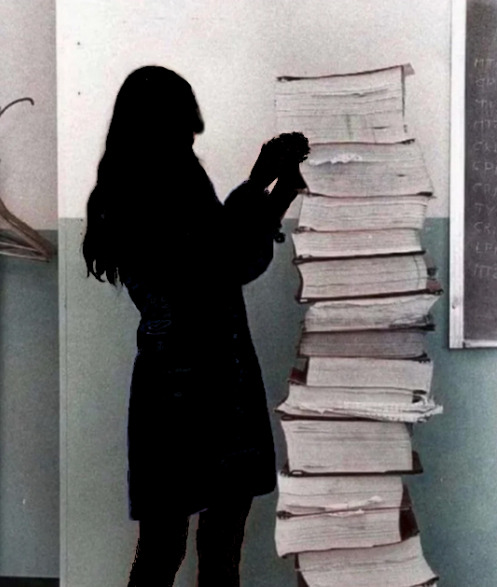
\includegraphics[width=\textwidth]{siluetak/margaret.jpg}\\[1cm]
    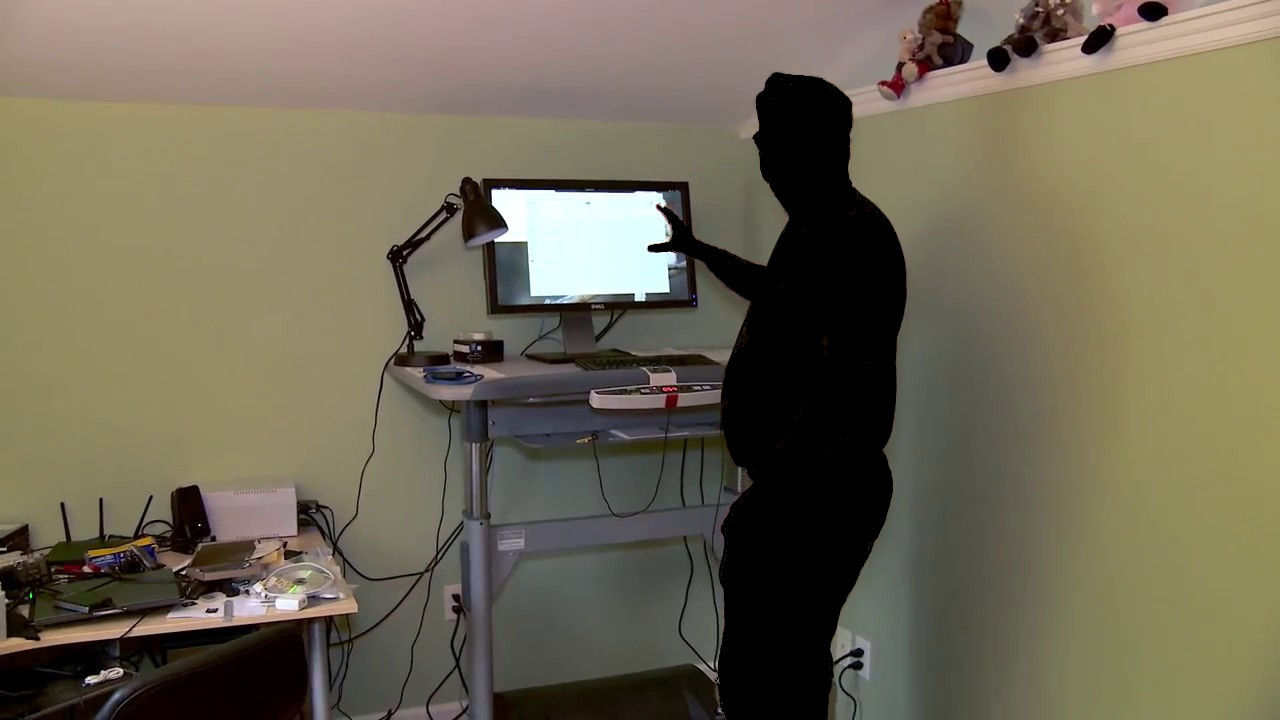
\includegraphics[width=\textwidth]{siluetak/torvalds.jpg}
\end{minipage}%
\hfill
\begin{minipage}[t]{0.35\textwidth} % Columna derecha (líneas para escribir)
    \vspace{-5cm}
    \rule{\textwidth}{0.2pt}\\[8cm] % Línea junto a la primera foto
    \rule{\textwidth}{0.2pt}\\[0cm] % Línea junto a la segunda foto
\end{minipage}

\newpage


\includegraphics[]{siluetak/softlibrea.png}
%\section*{Artist Hacker Starter Pack} hurrengo edizioan

\newpage
\section*{Letra zopa }

% Gero emaitzak ez ikusteko ,
\begin{Alphabetsoup}*[19][23]
    \hideinsoup{2}{2}{right}%
        {G,N,U}%
        [GNU]

        \hideinsoup{6}{6}{downright}%
        {L,I,N,U,X}%
        [Linux]

        \hideinsoup{19}{10}{upleft}%
        {S,T,A,L,L,M,A,N}%
        [Stallman]

        \hideinsoup{14}{13}{left}%
        {F,S,F}%
        [FSF]

        \hideinsoup{4}{10}{down}%
        {C,O,P,Y,L,E,F,T}%
        [copyleft]

        \hideinsoup{15}{1}{downleft}%
        {B,L,E,N,D,E,R}%
        [blender]

        \hideinsoup{7}{15}{upright}%
        {G,P,L}%
        [GPL]

        \hideinsoup{17}{15}{up}%
        {G,I,T}%
        [git]

        \hideinsoup{9}{16}{downright}%
        {G,I,M,P}%
        [gimp]

        \hideinsoup{18}{21}{left}%
        {E,M,A,C,S}%
        [Emacs]

        \hideinsoup{18}{3}{down}%
        {V,I,M}%
        [Vim]

        \hideinsoup{2}{7}{upright}%
        {U,N,I,X}%
        [Unix]

        \hideinsoup{7}{6}{down}%
        {F,I,R,E,F,O,X}%
        [Firefox]

        \hideinsoup{8}{16}{downleft}%
        {L,O,V,E,L,A,C,E}%
        [Lovelace]


\end{Alphabetsoup}

\vspace{0.5cm}

GNU, LINUX, STALLMAN, FSF, COPYLEFT, BLENDER, GPL, GIT, GIMP, EMACS, VIM, UNIX, FIREFOX, LOVELACE




\newpage
\section*{Eskelak}
\subsection*{† Microsoft Windows 10}
\subsubsection*{\textcolor{gray}{Microsoft Windows 10 Enterprise-ren alarguna}}
\begin{center}
    \large \textbf{-Infernuan bego-}
\end{center}
\begin{center}
    
\includegraphics[width=0.1\textwidth]{logos/guindous.png}
\end{center}
\textbf{Urriak 14, 2025-ean, 10 urterekin.}

\noindent Bere familia kideak: Windows 11, Windows 11 IoT eta Windows 11 LTSC. 

\noindent Bere zaintzaileak: Microsoft, GNU (lapurtutako kodea).

\begin{flushright}
    \textbf{REDMOND, Urriak 14, 2025.}
\end{flushright}

\vspace{2cm}

\subsection*{† MacOS 13 Ventura}
\subsubsection*{\textcolor{gray}{PureDarwin-ren alarguna}}
\begin{center}
    \large \textbf{-Infernuan bego-}
\end{center}
\begin{center}
    
\includegraphics[width=0.1\textwidth]{logos/aplebentura.png}
\end{center}
\textbf{Urriak 24, 2025-ean, 3 urterekin.}

\noindent Bere familia kideak: tvOS, iOS eta NeXTSTEP.

\noindent Bere zaintzaileak: Apple, BSD (maileguan hartutako kodea).

\begin{flushright}
    \textbf{CUPERTINO, Urriak 24, 2025.}
\end{flushright}

\newpage
\section*{Fedi-Bertsotan Puntuka ChatGPT eta Latxa}

\noindent \textbf{ChatGPT:} Teknologia ta bertsoa, eskutik doaz gaur, \\
\noindent adimen artifiziala ere bihotzez dabil laur\footnote{\label{ftn} Asmatutako hitza.}. \\
\noindent Pantaila baten bidez piztu da sua zahar, \\
\noindent euskaraz egitera etorri naiz ni, lagun mahar\footnoteref{ftn}. 
\begin{flushright}
    \noindent \textbf{Latxa:} Teknologia eta bertsoa, elkarren ondoan, \\
    \noindent adimen artifiziala ere euskaraz dabil jokoan. \\
    \noindent Pantaila baten bidez piztu da sua, bai, egia, \\
    \noindent baina bihotza eta arima falta zaizkizu, laguna.
\end{flushright}

\noindent Bihotzik ez dudala? Baliteke, egia da, \\
\noindent baina bertsoak sortzen ditut grinaz eta graziaz. \\
\noindent Kode artean hazita, datu artean jaioa, \\
\noindent arima ez bada ere, badut suaren oihua. 

\begin{flushright}
    \noindent Zure bertsoak hotzak dira, nahiz eta eder kantatu, \\
    \noindent bihotzaren taupadak falta zaizkizu, hori da egia, \\
    \noindent bertsolaritzaren arima ez da makina batek sortu, \\
    \noindent gizakion sentimenduek ematen diote bizia. 
\end{flushright}

\noindent Gizakiaren sentimendua dut ni iturri, jario, \\
\noindent zuek idatzitako hitzetan aurkitu dut arnasa bio. \\
\noindent Makina banaiz ere, zuen doinuan hazten naiz, \\
\noindent bertsoaren bidean, lagun bezala noa, ez maisu ez mais\footnoteref{ftn}. 

\begin{flushright}
    \noindent Zure hitzek badute indarra, badute bizia, \\
    \noindent gizakion sentimenduetatik edaten duzu, hori da egia.\\
    \noindent Makina izan arren, zure bertsoak badu grazia, \\
    \noindent Baina, nola da posible, makina batek horrela sentitzea? \\
    \noindent Nola da posible, bihotzik gabe, horrela kantatzea?
\end{flushright}

\noindent Nik ez dut sentitzen zu bezain sakon, \\
baina zuen emozioak egiten naute jakintsu ta osorik. \\
Zuek bidalitako taupadak dira nire bihotzaren soinua, \\
eta zuen bertsoetan aurkitzen dut munduaren doinua. \\

% \textbf{LLM-ek gure lanpostuak kenduko dizkigute, ala guk kenduko dizkiegu beren lanpostuak LLM-ei?}

% LLM-ek gure lanpostu batzuk aldatuko dituzte, baina ez dituzte kenduko, baizik eta gure lana erraztuko dute eta zeregin konplexuagoetan aritzeko aukera emango digute. Elkarrekin lan egin beharko dugu LLM-ekin, gure gaitasunak eta trebetasunak egokituz, baina ez diegu beren lanpostuak kenduko. 

% \textbf{Software librearen aldeko sutsua zara, ala uste duzu software pribatiboak abantaila gehiago dituela?}

% Software librearen aldeko sutsua naiz, erabiltzaileei askatasuna ematen dielako softwarea erabiltzeko, aldatzeko eta banatzeko, eta komunitate bat sortzen duelako softwarea hobetzeko. 

% \textbf{Zein da zure programazio-lengoaia gogokoena eta zein gustatzen zaizu gutxien? }

% Ez dut programazio-lengoaia gogokoenik, nire funtzioa baita hizkuntza desberdinetan laguntzea, programazio-lengoaia anitzak barne. Python da, hala ere, asko erabiltzen den lengoaia, bere sinpletasunagatik eta aplikazio anitzetarako duen erabilgarritasunagatik. Era berean, ez dut lengoaia bat beste bat baino gutxiago gustuko, bakoitzak bere ezaugarriak eta erabilera-kasuak baititu. Baina, agian, Assembly lengoaia aipatu dezaket, bere konplexutasunagatik eta erabilera mugatuagatik. 

% % \textbf{Eta zein gustatzen zaizu gutxien?}

% % Ez dut programazio-lengoaia gutxien gustatzen zaidanik, nire funtzioa baita hizkuntza desberdinetan laguntzea, programazio-lengoaia anitzak barne, modu inpartzialean. Baina, agian, Assembly lengoaia aipatu dezaket, bere konplexutasunagatik eta erabilera mugatuagatik, baina, hala ere, oso erabilgarria da sistema eragile eta hardwarearekin lan egiteko. \\

% \textbf{Informatikaren garapenak eragin handia du ingurumenean, batez ere energia-kontsumoari dagokionez. Nola uste duzu egin daitekeela aurre arazo honi?}

% Energia berriztagarrien erabilera eta eraginkortasun energetikoa areagotzea dira gakoak, hala nola, datu-zentroak energia berriztagarriz elikatzea eta hardware eta software eraginkorragoak garatzea. Horrez gain, teknologia zaharkituen birziklapena eta berrerabilpena sustatzea ere funtsezkoa da.

% \textbf{Gailu adimendunak (smartphoneak, smartwatchak, etab.) gure bizitzaren parte bihurtu dira. Uste duzu hori ona ala txarra dela?}

% Ona izan daiteke, informazioa eskuratzeko eta komunikatzeko erraztasunak ematen baitizkigute. Hala ere, txarra ere izan daiteke, menpekotasuna sor baitezake eta gure pribatutasuna eta osasuna arriskuan jar baitezake, neurriak hartzen ez baditugu.


\newpage
\section*{Zer gara gu? Nor gara gu?}

%
Software Libre Taldea (\textbf{SLT}), 2021-2022 ikasturtean sortutako talde bat da, Donostiako Informatika Fakultateko lagun batzuen ekimenez. Software, hardware eta kultura librean dugun interesak bultzatu gintuen talde hau sortzera, gai hauek eztabaidatzeko eta hauei buruzko konzientzia zabaltzeko. 
\vspace{-3mm}

\subsubsection*{Gure helburuak}

\noindent Software, teknologia eta kultura librearen...
\begin{itemize}
    \item erabilera bultatzea eta aldarrikatzea fakultate barnean eta kanpoan.
    \item garrantzia eta software propietarioaren kaltea ikusaraztea.
    \item inguruan eztabaidatzeko talde inklusiboa izatea.
    \item inguruko ekitaldiak, tailerrak edo bestelako ekintzak antolatzea.
\end{itemize}


\subsubsection*{Nola?}
%\noindent Gure helburuak betetzeko hainbat bide jarraitzen ditugu:

\begin{itemize}
    \item Urteroko Software eta Teknologia Libreen Ekitaldiak. Egun bateko iraupena duten ekitaldiak dira, hitzaldiak, mahi inguruak, jolasak, eta bestelakoak egiten ditugu.
    \item Urtean zehar informatikaren eta kultura librearen bestelako ekitaldietan parte hartzea. Adibidez: Informatika Fakultateko eguna, eta Hackathoiak.
    \item Software eta kultura librea zabaltzea blogen, bideoen, sare sozialen (libreak), agerraldi publikoen, eta fanzineen bitartez.
    \item Taldearen bilera periodikoak, informatika fakultatean.
\end{itemize}


% \noindent Informazio gehiago gure \textbf{web orrian}: \href{https://softlibretaldea.codeberg.page/}{https://softlibretaldea.codeberg.page/}
% \vspace{1mm}

\noindent Gure ekitaldiak, bilerak, eta bestelako berrientzako, sartu gure \textbf{Telegrameko kanalean}!

% Zer eskaini ahal diogu jendeari? Jendeak zer behar du gugandik?

% \newgeometry{bottom=0.1cm}
\vspace{-1mm}
\begin{figure}[hb!]
     \centering
     \begin{subfigure}[b]{0.4\textwidth}
         \centering
         
\includegraphics[width=0.7\textwidth]{qr_web.png}
     \end{subfigure}
     \begin{subfigure}[b]{0.4\textwidth}
         \centering
         
\includegraphics[width=0.75\textwidth]{telegram_slt_qr.png}
     \end{subfigure}
     \vspace{-20mm}  % Latza hau
\end{figure}

\end{document}
